\documentclass[12pt]{article}
%\usepackage[cp1251]{inputenc}
\usepackage[utf8]{inputenc}
\usepackage[bulgarian]{babel}
\usepackage{amssymb,amsmath,amsfonts,amstext,amscd,latexsym}
\usepackage{graphicx}
\usepackage{amsmath}
\usepackage[colorinlistoftodos]{todonotes}
\usepackage{systeme}
\usepackage[geometry]{ifsym}
\usepackage{listings}
\usepackage{float}
\usepackage{color}

\begin{document}
	\begin{titlepage}	
		\newcommand{\HRule}{\rule{\linewidth}{0.5mm}} % Defines a new command for the horizontal lines, change thickness here
		\center
		\textsc{\LARGE Софийски университет }\\[0.3cm]
		\textsc{\LARGE "Св. Климент Охридски" }\\[0.3cm]
		\textsc{\Large Факултет по математика и информатика }\\[0.2cm]
		%\fontsize{size}{baselineskip}
		
		{\fontsize{12}{18}\selectfont \bf МАШИННО САМООБУЧЕНИЕ}\vspace{15pt}\newline спец. Изкуствен интелект, I курс, зимен семестър \newline учебна година 2024/2025
		\vspace{30pt}
		
		
		
		
		\begin{minipage}{0.4\textwidth}
			\begin{flushleft}\large
				\emph{Изготвил:} \\
				Кристиян Симов \\ 
				фак. номер 4MI3400288
				%Попълнете вашето име, факултетен номер и група.
			\end{flushleft}
		\end{minipage}
		~
		%\begin{flushleft}
		\begin{minipage}{0.4\textwidth}
			\begin{flushright}
				\large
				\emph{Дата:}\\
				23. 10. 2024 г. % Попълнете датата на предаване
				\\София 
			\end{flushright}
		\end{minipage}\\[1cm]
		%\end{flushleft}
		\bigskip
		{\large \textbf{Домашна работа \textnumero 1}}\\[1cm] % Date, change the \today to a set date if you want to be precise
		%\includegraphics{rsz_sofia_university_logo.png}\\[1cm] 
		
\includegraphics{logo_su_no_text.png}\\[1cm]
		\vfill % Fill the rest of the page with whitespace
	\end{titlepage}
	
	
	
	\tableofcontents
	
	
	
	\newpage
	
	\section{Решение на задача \textnumero 1}
	
	Нека в контекста на изграждане на хипотези означим с $?$ - всички стойности на атрибут са възможни, а с $\varnothing$ - нито една не е възможна.\newline\newline
	Нека означим множествата с допустимите стойности (без $\varnothing$ и ?) за всеки от n-те атрибута с фамилията $ A = \{ A_{1}, A_{2}, ... ,  A_{n} \}$.\newline\newline
	Нека $m_{1} = |A_{1}|, m_{2} = |A_{2}|, ... , m_{n} = |A_{n}|$\newline\newline
	Тогава за задачата от Лекция 1 имаме $m_{1} = 3, m_{2} = 2, ..., m_{6} = 2$\newline\newline
	По вероятностни съображения, тъй като можем да избираме първо по 3 начина, после по 2, ... , накрая отново по 2, получаваме, че броя на всички различни възможни примери е точно числото:
	\[E_{6} = \displaystyle \prod_{i = 1}^6 m_{i} = 3 * 2^{5} = 3 * 32 = 96\]
	За броя на възможните хипотези, които в тази задача имат вида $\langle a_{1},...,a_{6} \rangle$, където $a_{i} \in A_{i}$ или $a_{i}=?$, или $a_{i}=\varnothing$, правим аналогично съображение на предходното, но към всяка мощност $m_{i}$ трябва да прибавим 2 (броим ? и $\varnothing$, като валидни стойности за $a_{i}$). Така бихме получили: \[\displaystyle \prod_{i = 1}^6(m_{i}+2) = 5*4^{5} = 5 * 1024 = 5120,\] но ще преброим всеки вектор $\langle a_{1},...,a_{6} \rangle$, където за някое $i$ имаме $a_{i} = \varnothing$. \newline Тези вектори за нашите цели ефективно са като вектора $\langle\varnothing, \varnothing,..., \varnothing\rangle$ и затова нека преброим само него и към броя възможности прибавяме само 1-ца (за $?$). Така броя на различните възможни хипотези спада на едва: \[H_{6} = 1 + \displaystyle \prod_{i = 1}^6(m_{i}+1) = 1 + 4*3^{5} = 1 + 4*243 = 1+ 972 = 973\]\newline\newline
	Нека добавим множество $A_{7}$ с мощност $m_{7}=3$ (по условие) към фамилията $A$. Тогава вече ще имаме брой възможни примери равен на: \[E_{6}*m_{7} = (\displaystyle \prod_{i = 1}^6 m_{i})*m_{7} = \displaystyle \prod_{i = 1}^7 m_{i} = 96*3 = 288\] От своя страна, броят хипотези ще се измени по следния начин: \[1 + (\displaystyle \prod_{i = 1}^6 (m_{i}+1))*(m_{7}+1) = 1 + 972*4 = 1 + 3888 = 3889\] Или изразено чрез $H_{6}$: \[1 + (H_{6} -  1) * (m_{7}+1) = H_{6} * (m_{7}+1) - m_{7} = 973*4 - 3 = 3892 - 3 = 3889\]\newline\newline
	Нека по-общо прибавим $(n+1)$-во множество $A_{n+1}$ ($\varnothing \notin A_{n+1}$ и  $? \notin A_{n+1}$)  \newline с мощност $k$, т.е. $m_{n+1} =|A_{n+1}|=k$, към фамилията $A$. \newline\newline 
	Тогава ако функцията $E_{n} = E(n)$ описва нарастването на броя възможни примери, а $H_{n} = H(n)$ - на броя възможни хипотези то:\newline \newline $E(n+1) = E(n)*m_{n+1} = E(n)*k$ \newline $H(n+1) = H(n)*(m_{n+1}+1) - m_{n+1} = H(n)*(k+1) - k$
	
	\newpage
	
	
	\section{Решение на задача \textnumero 2}
	
	Нека в множество D имаме обучаващи примери от вида $\langle x, c(x) \rangle$, които в зависимост от реда на постъпване при обучението са индексирани по следния начин (в обратен ред спрямо таблицата от Лекция 1):
		\subparagraph{}
		$x_{1} = \langle $ \textit{Слънце, Топъл, Висока, Силен, Студена, Промяна} $\rangle  +$
		\subparagraph{}
		$x_{2} = \langle $ \textit{Дъжд, Студен, Висока, Силен, Топла, Промяна} $\rangle  -$
		\subparagraph{}
		$x_{3} = \langle $ \textit{Слънце, Топъл, Висока, Силен, Топла, Същото} $\rangle  +$
		\subparagraph{}
		$x_{4} = \langle $ \textit{Слънце, Топъл, Нормална, Силен, Топла, Същото} $\rangle  +$
	\newline\newline
	Тогава алгоритъмът CANDIDATE-ELIMINATION ще премине през следните стъпки:\newline
	
	
	\paragraph{0)} Инициализация
		\subparagraph{}
		$G_{0} \leftarrow \langle $ \textit{?, ?, ?, ?, ?, ?} $\rangle$ 
		\subparagraph{} 
		$S_{0} \leftarrow \langle  \varnothing, \varnothing, \varnothing, \varnothing, \varnothing, \varnothing \rangle$
	
	\paragraph{1)} $x_{1} = \langle $ \textit{Слънце, Топъл, Висока, Силен, Студена, Промяна} $\rangle  +$ \newline\newline
	Примерът е положителен. В $G_{0}$ няма несъвместими хипотези, остава както е. $S_{0}$ е несъвместима, тъй като е твърде специфична, премахваме я. В съответствие с $x_{1}$ добавяме хипотеза $s_{1}$ към $S_{1}$.
		\subparagraph{}
		$S_{1} \leftarrow \langle $ \textit{Слънце, Топъл, Висока, Силен, Студена, Промяна} $ \rangle$
		\subparagraph{}
		$G_{1} \leftarrow G_{0}$
		
	\paragraph{2)} $x_{2} = \langle $ \textit{Дъжд, Студен, Висока, Силен, Топла, Промяна} $\rangle  -$ \newline\newline
	Примерът е отрицателен. В $S_{1}$ няма несъвместими хипотези, остава както е. $G_{1}$ е несъвместима, тъй като е твърде обща, премахваме я. В съответствие с $x_{2}$ и $S_{2}$ добавяме само хипотези $g_{2.1}$, $g_{2.2}$ и $g_{2.5}$ към $G_{2}$:
		\subparagraph{}
		$S_{2} \leftarrow S_{1}$
		\subparagraph{} 
		$G_{2} \leftarrow \langle $ \textit{Слънце, ?, ?, ?, ?, ?} $ \rangle$
		\subparagraph{} 
		$G_{2} \leftarrow \langle $ \textit{?, Топъл, ?, ?, ?, ?} $ \rangle$
		\subparagraph{} 
		$G_{2} \leftarrow \langle $ \textit{?, ?, ?, ?, Студена, ?} $ \rangle$
	
	\paragraph{3)} $x_{3} = \langle $ \textit{Слънце, Топъл, Висока, Силен, Топла, Същото} $\rangle  +$ \newline\newline
	Примерът е положителен. $S_{2}$ е несъвместима, тъй като е твърде специфична. Обобщаваме единствената хипотеза в нея до $s_{3}$ и получаваме $S_{3}$. Вече хипотезата $g_{2.5}$ от $G_{2}$ е несъвместима с резюмето $s_{3}$ на всички положителни примери до този момент, премахваме я от $G_{2}$ и получаваме $G_{3}$.
		\subparagraph{}
		$S_{3} \leftarrow \langle $ \textit{Слънце, Топъл, Висока, Силен, ?, ?} $ \rangle $
		\subparagraph{} 
		$G_{3} \leftarrow G_{2} \setminus \langle $ \textit{?, ?, ?, ?, Студена, ?} $ \rangle$
		
	\paragraph{4)} $x_{4} = \langle $ \textit{Слънце, Топъл, Нормална, Силен, Топла, Същото} $\rangle  +$ \newline\newline
	Примерът е положителен. $S_{3}$ е несъвместима, тъй като е твърде специфична. Обобщаваме единствената хипотеза в нея до $s_{4}$ и получаваме $S_{4}$. Новополученото резюме $s_{4}$ е съвместимо с хипотезите от $G_{3}$. Следователно за $G_{4}$ получаваме $G_{3}$.
		\subparagraph{}
		$S_{4} \leftarrow \langle $ \textit{Слънце, Топъл, ?, Силен, ?, ?} $ \rangle $
		\subparagraph{} 
		$G_{4} \leftarrow G_{3} = \{ \langle $ \textit{Слънце, ?, ?, ?, ?, ?} $ \rangle, \langle $ \textit{?, Топъл, ?, ?, ?, ?} $ \rangle \}$
	\newline
	Очаквано, получихме същия резултат като при $x_{4}$ $\rightarrow$ $x_{3}$ $\rightarrow$ $x_{2}$ $\rightarrow$ $x_{1}$. $\square$
	
	
	
	\newpage
	
	\section{Решение на задача \textnumero 3}
	
	Нека бележим хипотезите (правоъгълниците) по следния съкратен начин:
		\subparagraph{}
		$h_{\square} = \langle a, b, c, d \rangle$
		
		\paragraph{}
	Да приемем, че всичките обучаващи примери (както и бъдещи примери за класификация) се побират в двумерно пространство на характеристиките (атрибутите) с размерност 10 на 10, център $(0, 0)$ и дискретни стойности - единствено положителни цели числа.
	
	\paragraph{}
	Нека в множество D имаме обучаващи примери от вида $\langle x, c(x) \rangle$, които в зависимост от реда на постъпване при обучението са индексирани по следния начин (напълно произволно, с изключение на това че първо са индексирани положителните примери, с цел стегнатост на решението - ако имаме резюмето на положителните по начало, ще можем с лекота да отхвърлим множество от хипотези за G):
	
		\subparagraph{}
		$x_{1} = \langle $ 6, 5 $\rangle  +$
		\subparagraph{}
		$x_{2} = \langle $ 5, 3 $\rangle  +$
		\subparagraph{}
		$x_{3} = \langle $ 4, 4 $\rangle  +$
		\subparagraph{}
		$x_{4} = \langle $ 5, 1 $\rangle  -$
		\subparagraph{}
		$x_{5} = \langle $ 1, 3 $\rangle  -$
		\subparagraph{}
		$x_{6} = \langle $ 2, 6 $\rangle  -$
		\subparagraph{}
		$x_{7} = \langle $ 5, 8 $\rangle  -$
		\subparagraph{}
		$x_{8} = \langle $ 9, 4 $\rangle  -$
	

	
	\paragraph{}
	Тогава алгоритъмът CANDIDATE-ELIMINATION ще премине през следните стъпки:\newline
	
	
	\paragraph{0)} Инициализация
		\subparagraph{}
		$S_{0} \leftarrow \langle \varnothing, \varnothing, \varnothing, \varnothing \rangle$
		\subparagraph{}
		$G_{0} \leftarrow \langle 0, 10, 0, 10 \rangle$
		
	\paragraph{1)} $x_{1} = \langle $ 6, 5 $\rangle  +$
	\paragraph{}
	Примерът е положителен. $G_{0}$ е съвместима. $S_{0}$ е твърде специфична, тъй като е несъвместима. Обобщаваме я и получаваме $S_{1}$ - правоъгълник, който покрива точно една точка - самата $x_{1}$.
		\subparagraph{}
		$S_{1} \leftarrow \langle 6, 6, 5, 5 \rangle$
		\subparagraph{}
		$G_{1} \leftarrow G_{0}$
		
	\paragraph{2)} $x_{2} = \langle $ 5, 3 $\rangle  +$
	\paragraph{}
	Примерът е положителен. $G_{1}$ е съвместима. Остава както е. $S_{1}$ е твърде специфична и значи несъвместима. Обобщаваме я и получаваме $S_{2}$ - правоъгълник, който покрива точно двете точки $x_{1}$ и $x_{2}$.
		\subparagraph{}
		$S_{2} \leftarrow \langle 5, 6, 3, 5 \rangle$
		\subparagraph{}
		$G_{2} \leftarrow G_{1}$
		
	\paragraph{3)} $x_{3} = \langle $ 4, 4 $\rangle  +$
	\paragraph{}
	Примерът е положителен. $G_{2}$ е съвместима. Остава както е. $S_{2}$ е твърде специфична и значи несъвместима. Обобщаваме я и получаваме $S_{3}$ - правоъгълник, който покрива точно трите точки $x_{1}$, $x_{2}$ и $x_{3}$.
		\subparagraph{}
		$S_{3} \leftarrow \langle 4, 6, 3, 5 \rangle$
		\subparagraph{}
		$G_{3} \leftarrow G_{2}$
	
	\paragraph{4)} $x_{4} = \langle $ 5, 1 $\rangle  -$
	\paragraph{}
	Примерът е отрицателен. $S_{3}$ е съвместима. Остава както е. $G_{3}$ е твърде обща и значи несъвместима. Специфицираме я и получаваме $g_{4}$ - единствен правоъгълник, който е съвместим едновременно с $S_{3}$ и с новата точка $x_{4}$.
		\subparagraph{}
		$S_{4} \leftarrow S_{3}$
		\subparagraph{}
		$G_{4} \leftarrow \langle 0, 10, 2, 10 \rangle$
	
	\paragraph{5)} $x_{5} = \langle $ 1, 3 $\rangle  -$
	\paragraph{}
	Примерът е отрицателен. $S_{4}$ е съвместима. Остава както е. $G_{4}$ е твърде обща и значи несъвместима. Специфицираме я и получаваме $g_{5}$ - единствен правоъгълник, който е съвместим едновременно с $S_{4}$ и с новата точка $x_{5}$.
		\subparagraph{}
		$S_{5} \leftarrow S_{4}$
		\subparagraph{}
		$G_{5} \leftarrow \langle 2, 10, 2, 10 \rangle$
		
	\paragraph{6)} $x_{6} = \langle $ 2, 6 $\rangle  -$
	\paragraph{}
	Примерът е отрицателен. $S_{5}$ е съвместима. Остава както е. $g_{5}$ от $G_{5}$ е твърде обща и значи несъвместима. Специфицираме я и получаваме $g_{6.1}$ и $g_{6.2}$- два възможни правоъгълника, който са съвместими едновременно с $S_{5}$ и с новата точка $x_{6}$.
		\subparagraph{}
		$S_{6} \leftarrow S_{5}$
		\subparagraph{}
		$G_{6} \leftarrow \{ \langle 3, 10, 2, 10 \rangle,\langle 2, 10, 2, 5 \rangle \}$
		
	\paragraph{7)} $x_{7} = \langle $ 5, 8 $\rangle  -$
	\paragraph{}
	Примерът е отрицателен. $S_{6}$ е съвместима. Остава както е. $g_{6.1}$ от $G_{6}$ е твърде обща и значи несъвместима. Специфицираме я и получаваме $g_{7.2}$, a $g_{7.1}$ е съвместимата $g_{6.2}$ от $G_{6}$. Накрая, в $G_{7}$ имаме единствено два възможни правоъгълника, който са съвместими едновременно с $S_{6}$ и с новата точка $x_{7}$.
	\subparagraph{}
	$S_{7} \leftarrow S_{6}$
	\subparagraph{}
	$G_{7} \leftarrow (G_{6}\setminus\{3,10,2,10\}) \cup  \{ \langle 3, 10, 2, 7 \rangle \}$
	\subparagraph{}
	$G_{7} = \{ \langle 2, 10, 2, 5 \rangle,\langle 3, 10, 2, 7 \rangle \}$
	
	\paragraph{8)} $x_{8} = \langle $ 9, 4 $\rangle  -$
	\paragraph{}
	Примерът е отрицателен. $S_{7}$ е съвместима. Остава както е. $g_{7.1}$ и $g_{7.2}$ от $G_{7}$ са твърде общи и значи несъвместими. Специфицираме ги и получаваме $g_{8.1}$ и $g_{8.2}$ - два възможни правоъгълника, който са съвместим едновременно с $S_{7}$ и с новата точка $x_{8}$.
	\subparagraph{}
	$S_{8} \leftarrow S_{7} (= S_{6} = ... = S_{3} = \langle 4, 6, 3, 5 \rangle)$
	\subparagraph{}
	$G_{8} \leftarrow \{ \langle 2, 8, 2, 5 \rangle,\langle 3, 8, 2, 7 \rangle \}$
	\newline\newline
	Край на обучението.
	\newpage
	
	\begin{figure}[H]
		\centering
		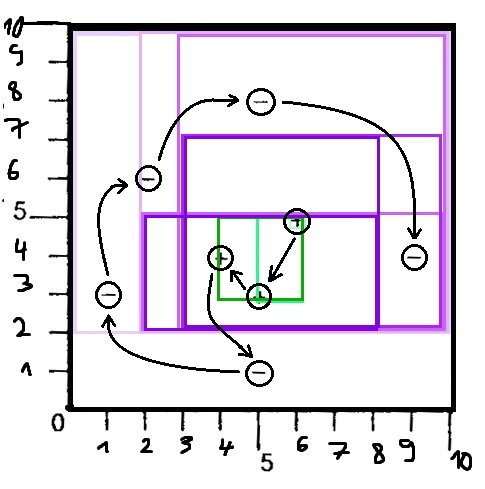
\includegraphics[width=130mm]{Untitled.jpg} 
		\caption{На изображението виждаме в нюансите на зеления цвят последователните хипотези за S, а в нюансите на лилавото - последователните хипотези за G, генерирани в хода на изпълнението на алгоритъма. Финалните хипотези са нанесени в съответните най-тъмни нюанси.}
	\end{figure}
	\newpage
	
	\subsection{}
	Финалния вид на S след обучението е следния:
	\paragraph{}
	$S = \langle 4, 6, 3, 5 \rangle$
	\newline\newline
	Видът на S e нанесен в най-тъмния нюанс на зеленото на чертежа в Фиг.1 на стр.10
	
	\subsection{}
		Финалния вид на G след обучението е следния:
	\paragraph{}
	$G = \{ \langle 2, 8, 2, 5 \rangle,\langle 3, 8, 2, 7 \rangle \}$
	\newline\newline
	Видът на G e нанесен в най-тъмния нюанс лилавото на чертежа в Фиг.1 на стр.10
	
	\subsection{}
	
	Нека хипотезите от $G = \{ \langle 2, 8, 2, 5 \rangle,\langle 3, 8, 2, 7 \rangle \}$ означим такa:
		\subparagraph{}
		$g_{1} = \langle 2, 8, 2, 5 \rangle$
		\subparagraph{}
		$g_{2} = \langle 3, 8, 2, 7 \rangle$
	\newline\newline
	Тогава пример, който ще намали пространството на версиите задължително когато постъпи, се намира в участъка $\langle 3, 8, 5, 7 \rangle$ (в $g_{2}$, но извън $g_{1}$), например нека това е:
		\subparagraph{}
		$x_{decr} = \langle 4,6 \rangle$
	
	\paragraph{1.1)} $x_{decr} = \langle 4,6 \rangle +$ \newline\newline
	Примерът е положителен. Тогава хипотезата $g_{1}$ вече няма да е съвместима с него и ще трябва да я премахнем. В допълнение ще трябва да обобщим единствената хипотеза $s_{1}$ от $S$, така че тя да покрие новия положителен пример, което обаче няма да промени броят хипотези. В крайна сметка броят хипотези намалява (съответно и пространството на версиите).
	
	\paragraph{1.2)} $x_{decr} = \langle 4,6 \rangle -$ \newline\newline
	Примерът е отрицателен. Тогава хипотезата $g_{2}$ вече няма да е съвместима с него и ще трябва да я премахнем, тъй като тя ще се специфицира до нова хипотеза $g_{3}$, която попада изцяло вътре в $g_{1}$. Така в крайна сметка в $G$ ще остане само $g_{1}$. Следователно отново правим същия извод като в края на 1.1).
	\newline
	\newline
	\newline
	Пример, който няма да намали пространството на версиите задължително когато постъпи, се намира в участъка извън пространството заключено от $G$, например нека това е:
	\subparagraph{}
	$x_{\neg decr} = \langle 9,4 \rangle$
	
	\paragraph{2.1)} $x_{\neg decr} = \langle 9,4 \rangle -$ \newline\newline
	Примерът задължително ще е отрицателен, според модела нямаме друг случай за него. Той е съвместим и с $S$, и с $G$. Следователно няма нужда да правим промени по хипотезите и така пространството на версиите не се променя (тоест също така не намалява).
	
	
	\subsection{}
	
	По дефиниция, за да се научи едно понятие абсолютно точно, е необходимо границите S и G да се ``стегнат'' до една и съща граница съдържаща единствена хипотеза.\newline\newline
	В случая искаме това да е точно хипотезата:
	\paragraph{}
	$h_{\square} = \langle 3, 5, 2, 9 \rangle$\newline\newline
	
	\paragraph{1)}
	Първо да конструираме S, която има същия вид като $h_{\square}$.\newline\newline
	За целта можем да използваме минимално 2 обучаващи положителни примера, които ако свържем биха образували диагонала на хипотезата (правоъгълника 	$h_{\square}$), например:
		\subparagraph{}
		$x_{1} = \langle $ 3, 2 $\rangle  +$ и $x_{2} = \langle $ 5, 9 $\rangle  +$
	\paragraph{}
	Така ще получим $S_{2} = \langle 3, 5, 2, 9 \rangle$ за две стъпки от $S_{0} = \langle \varnothing,\varnothing,\varnothing,\varnothing \rangle$:
		\subparagraph{}
		$\langle \varnothing,\varnothing,\varnothing,\varnothing \rangle \rightarrow \langle 3,3,2,2 \rangle \rightarrow \langle 3,5,2,9 \rangle$
	
	\paragraph{2)}
	Сега остана да ``свиваме'' $G$ докато $G \equiv S$.\newline\newline
	За целта можем да използваме минимално 4 обучаващи отрицателни примера, които заради стъпка 1) е нужно да са непосредствено извън $S_{2}$ и разположени перпендикулярно над средите на всяка от страните на правоъгълника $h_{\square}$, с цел несъвместимите спецификации на $G$ да се отхвърлят възможно най-рано, тъй като по-този начин отрицателните примери ще попадат непосредствено между двата положителни формиращи $h_{\square}$. Нека например това са:
		\subparagraph{}
		$x_{3} = \langle $ 2, 5 $\rangle  -$, $x_{4} = \langle $ 4, 1 $\rangle  -$, $x_{5} = \langle $ 6, 5 $\rangle  -$ и $x_{6} = \langle $ 4, 10 $\rangle  -$\newline\newline
		
	
	Така ще получим $G_{4} = \langle 3, 5, 2, 9 \rangle$ за четири стъпки от $G_{0} = \langle 0,10,0,10 \rangle$:
		\subparagraph{}
		$\langle 0,10,0,10\rangle \rightarrow \langle 3,10,0,10 \rangle \rightarrow \langle 3,10,2,10 \rangle \rightarrow \langle 3,5,2,10 \rangle \rightarrow \langle 3,5,2,9 \rangle$
	\newline\newline\newline
	Визуално пояснение на гореизложенето в 1) и 2) може да бъде видяно във Фиг.2 на стр.14 (следващата и последна страница).

	\newpage
	\begin{figure}[H]
		\centering
		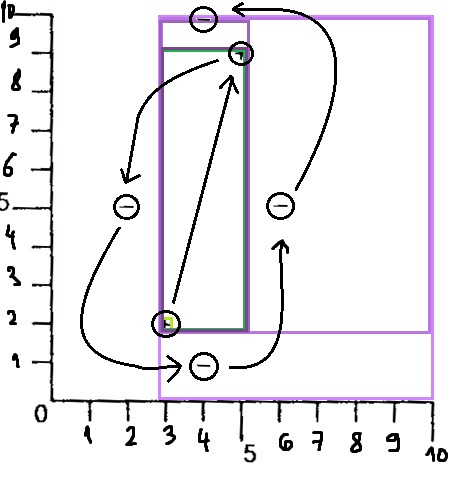
\includegraphics[width=130mm]{Untitled3.jpg} 
		\caption{На изображението виждаме в нюансите на зеления цвят последователните хипотези за S, а в нюансите на лилавото - последователните хипотези за G, генерирани в хода на изпълнението на построението от 1) и 2). Забелязваме, че поставяйки отрицателните примери в определени геометрични среди, те бързо разрязват пространството максимизирайки скоростта на обучение. Финалните хипотези за S и G са нанесени в съответните най-тъмни нюанси. Както се вижда те ще съвпаднат, както искахме, и то с минималния брой от 6 необходими точки - 2 положителни за S и 4 отрицателни за G.}
	\end{figure}
	
	
	
	
\end{document}